\documentclass[11pt,a4paper]{article}
\usepackage[T1]{fontenc}
\usepackage[utf8]{inputenc}
\usepackage{lmodern}
\usepackage{amsmath,amssymb,amsthm,mathtools,mathrsfs}
\usepackage{graphicx,float,xcolor,multicol}
\usepackage[shortlabels]{enumitem}
\usepackage[margin=27mm]{geometry}
\usepackage{microtype,needspace,placeins}
\usepackage{tikz,tikz-cd}
\usetikzlibrary{arrows.meta,calc,positioning,patterns,decorations.pathreplacing}
\usepackage[colorlinks=true,linkcolor=teal,urlcolor=teal,citecolor=teal]{hyperref}
\setlength{\parindent}{0pt}
\setlength{\parskip}{.6em}
\setcounter{secnumdepth}{0}
\allowdisplaybreaks
\raggedbottom
\providecommand{\cross}{\times}
\DeclareUnicodeCharacter{2020}{\ensuremath{\dagger}}
\DeclareMathOperator{\supp}{supp}
\DeclareMathOperator*{\esssup}{ess\,sup}
\providecommand{\chapter}{\section}
\newenvironment{tool}[2]{\subsection*{Tool #1 --- #2}}{}
\newcommand{\ToolRef}[1]{Tool #1}
\newcommand{\FigureTag}[2]{\textit{Figure #1}}
\newcommand{\Result}[1]{\subsection*{#1}}
\newcommand{\Application}[1]{\subsubsection*{Application\if\relax\detokenize{#1}\relax\else\space--- #1\fi}}
\newcommand{\ProofHeading}{\par\textit{Proof.}\space}
\newcommand{\ProofOf}[1]{\par\textit{Proof of #1.}\space}
\newcommand{\RemarkHeading}{\par\textbf{Remark.}\space}
\newcommand{\NoteHeading}{\par\textbf{Note.}\space}
\newcommand{\ExerciseHeading}{\par\textbf{Exercise.}\space}

\graphicspath{{figures/complex-analysis/}}
\begin{document}
\section*{Winding Number}
% BLOG-CONTENT-BEGIN
Let us look at singularities through contour integration.

\subsection*{Recall: Cauchy's Theorem}
If \(\gamma_0:[0,1]\to U\) and \(\gamma_1:[0,1]\to U\) are two closed rectifiable curves and \(f\in H(U)\), then
\[
  \int_{\gamma_0} f(z)\,dz=\int_{\gamma_1} f(z)\,dz.
\]

One thing that the complex tube lemma ensures is that there is always a rectifiable curve (a polygonal path) in a small enough tube (hence in \(U\)) of any continuous curve. Thus, we can extend our definition of integration to any continuous curve (our holomorphic function will not mind).


Therefore, for \(f\in H(U)\) and \(\gamma:[0,1]\to U\) continuous, we define
\[
  \int_\gamma f(z)\,dz:=\int_{\gamma'} f(z)\,dz,
\]
where \(\gamma'\) is rectifiable and homotopic to \(\gamma\).

Checking that this is well-defined is important and not so difficult. Let \(f\in H(U_1)\), \(\gamma\sim\gamma_1\), and let \(f\in H(U_2)\), \(\gamma\sim\gamma_2\), where \(\gamma_i\subset U_i\). Let \(\gamma_P\) be a polygonal path in a small enough tube such that \(\gamma_P\subset U_1\cap U_2\) and \(\gamma_P\sim\gamma\). Then \(\gamma_P\sim\gamma_1\) and \(\gamma_P\sim\gamma_2\), in \(U_1\) and \(U_2\), respectively. Since \(f\in H(U_1\cup U_2)\) and \(\gamma_1\sim\gamma_2\) in \(U_1\cup U_2\), we have
\[
  \int_{\gamma_1} f(z)\,dz
  =\int_{\gamma_2} f(z)\,dz
  =\int_\gamma f(z)\,dz.
\]
Thus, our definition is independent of the domain and the specific choice of rectifiable curve.

But even now, functions integrated on different equivalence classes would yield different values. Let us eliminate this possibility too by demanding our domain \(U\) to be simply connected. Note here that if \(\gamma:[0,1]\to U\) is any closed curve, then
\[
  \int_\gamma f(z)\,dz=0.
\]
Let us now spike the function \(f\) with a singularity at \(z_0\) by considering
\[
  \frac{H(z)}{z-z_0}.
\]
We know locally that \(H(z)=H(z_0)+(z-z_0)f'(z_0)+\cdots,\)
and hence
\[
  \frac{H(z)-H(z_0)}{z-z_0}=f'(z_0)+\cdots=:g(z).
\]
We know that \(g\) is holomorphic near \(z_0\), but can we say something about \(g\) globally? If we can somehow say that \(g\) is holomorphic, then
\[
  \int_\gamma \frac{H(z)-H(z_0)}{z-z_0}\,dz
  =\int_\gamma g(z)\,dz=0,
\]
so
\[
  \int_\gamma \frac{H(z)}{z-z_0}\,dz
  =H(z_0)\int_\gamma \frac{dz}{z-z_0}.
\]


Let us first focus on
\[
  g(z)=\frac{H(z)-H(z_0)}{z-z_0}.
\]
Clearly, \(g\in H(U\setminus\{z_0\})\) and is bounded near \(z_0\), which can be seen from the linear approximation of \(f\) near \(z_0\).

\paragraph{Digression.}
Suppose \(f\in H(U\setminus\{z_0\})\) and \(f\) is bounded near \(z_0\). Let \(\overline{B_r(z_0)}\subset U\), and let \(\gamma\) and \(\gamma'\) be two circles in \(B_r(z_0)\). As \(B_r(z_0)\) is convex, we have
\[
  \int_\gamma f(z)\,dz=\int_{\gamma'} f(z)\,dz.
\]
Now, if we estimate,
\[
  \left|\int_{\gamma'} f(z)\,dz\right|<M,2\pi\varepsilon
  \qquad(\forall\varepsilon,\ \varepsilon>0),
\]
where \(M\) is a bound for \(f\) and \(\varepsilon\) is the radius of \(\gamma'\). Thus, \(f\) vanishes on closed paths near \(z_0\), and hence is conservative near \(z_0\).

But \(f\) is continuous in \(\overline{B_r(z_0)}\setminus\{z_0\}\), which is not compact, so \(f\) need not be uniformly continuous. To sidestep this, define
\[
  F(z):=\int_{\gamma_{z^*\to z}} f(z)\,dz,
\]
where \(\gamma_{z^*\to z}\) is some polygonal path in \(U\setminus\{z_0\}\) and \(z^*\in U\setminus\{z_0\}\). First note that \(F\in H(U\setminus\{z_0\})\). As the polygonal path can be written as line segments,
\[
  F=\sum_{k=0}^{N}\int_{a_k}^{a_{k+1}} f(s,z)\,ds,
\]
where \(\gamma_{z^*\to z}|_{[a_k,a_{k+1}]}\) is a line segment and

\[
  f(s,z)=f\circ\gamma_{z^*\to z}|_{[a_k,a_{k+1}]}\,b_k,
\]
where \(b_k\) is the slope of the segment. From a statement proved previously, \(F\in H(U\setminus\{z_0\})\). Also,
\[
  |F(z+h)-F(z)|
  =\left|\int_{\gamma_{z\to z+h}}f(z)\,dz\right|
  \le M\,|\gamma_{z\to z+h}|=M|h|.
\]
Thus, \(F\) is uniformly continuous in \(U\setminus\{z_0\}\), and therefore \(F\) can be continuously extended to \(z_0\).


For \(z\) close to \(z^*\),
\[
  |F(z)|\le \int_{\gamma_{z^*\to z}}|f(z)|\,dz
  \qquad\text{in }B_\varepsilon(z^*)\subset U.
\]
Thus, \(F\) is bounded near \(z^*\) and \(z_0\). By a similar argument, we can conclude that \(F\) vanishes on contours that are closed. By Morera, \(F\in H(U)\), and therefore \(F'=f\in H(U)\).

Replacing \(f\) with \(g\), we see that \(g(z)=\frac{H(z)-H(z_0)}{z-z_0}\)
is holomorphic on \(U\).

\textbf{Note.}
The reason we yearn for uniform continuity is that the image of a Cauchy sequence is Cauchy: if \(x_n\to x\), then \(f(x_n)\to f(x)\); moreover, if \(y_n\to x\), then \(f(y_n)\to f(x)\). This property helps us extend functions and fill gaps in their domains.

Finally, for any closed curve \(\gamma\) in \(U\), with \(z_0\notin\gamma([0,1])\), we have
\[
  \frac{1}{2\pi i}\int_\gamma\frac{H(z)}{z-z_0}\,dz
  =\left(\frac{1}{2\pi i}\int_\gamma\frac{dz}{z-z_0}\right)H(z_0).
\]
This terse generalization of the Cauchy Integral Formula leaves us with a rather intelligent integral:
\[
  \frac{1}{2\pi i}\int_\gamma\frac{dz}{z-z_0},
  \qquad z_0\notin\gamma([0,1]).
\]
The reason we think so is that, given any continuous closed curve (let us assume injectivity for simplicity), we intuitively have an


idea of what is ``inside'' \(\gamma\) and what is outside. Let
\[
  \operatorname{dist}(z_0,\gamma):=\inf_t|z_0-\gamma(t)|=d>0.
\]

\begin{figure}[htbp]
  \centering
  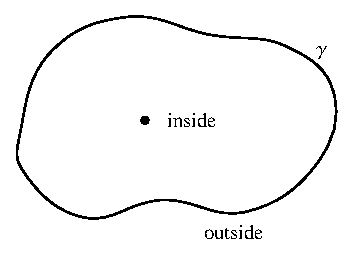
\includegraphics[width=.38\linewidth]{note5-fig-01.pdf}

\end{figure}

Then, by the complex tube lemma, we can find a polygonal path \(\gamma_P\) such that \(|\gamma(t)-\gamma_P(t)|<d.\)
Recall again that, by the very construction of \(\gamma_P\), there is a straight-line homotopy, piecewise, between \(\gamma\) and \(\gamma_P\). Concatenate these to obtain a piecewise homotopy function
\[
  \overline{\gamma}:[0,1]\times[a_k,a_{k+1}],
  \qquad
  \overline{\gamma}(s,t)=(1-s)\gamma(t)+s\gamma_P(t).
\]
Since
\[
  |\gamma(t)-\gamma_P(t)|<d<|\gamma(t)-z_0|,
\]
we have \(z_0\notin\operatorname{im}(\overline{\gamma})\), for all pieces
\[
  0=a_0<a_1<a_2<\cdots<a_n=1.
\]
Therefore,
\[
  \int_\gamma\frac{dz}{z-z_0}
  =\int_{\gamma_P}\frac{dz}{z-z_0}.
\]
Now we know what the interior of a closed polygonal, simple path is. Thus, if \(z_0\) is in the interior,
\[
  \int_{\gamma_P}\frac{dz}{z-z_0}=1
\]
by the Cauchy Integral Formula, and if \(z_0\) is in the exterior of \(\gamma_P\), then
\[
  \int_{\gamma_P}\frac{dz}{z-z_0}=0
\]
by Cauchy's theorem. Hence,
\[
  \int_\gamma\frac{dz}{z-z_0}
  =\int_{\gamma_P}\frac{dz}{z-z_0}
  =1\text{ or }0,
\]
based on where \(z_0\) is. There is good reason to believe that this integral captures the notion of interior and exterior. But does this integral


also capture the notion of interior and exterior topologically? That is, given any \(z_0\) in the ``interior'' of \(\gamma\), can we also say that there exists \(\varepsilon>0\) such that \(B_\varepsilon(z_0)\) is also in the ``interior'' of \(\gamma\)? The answer is affirmative here too.

If we define
\[
  \gamma'(t)=\gamma(t)-h,
  \qquad h<d=\operatorname{dist}(\gamma(t),z_0),
\]
and again consider the straight-line homotopy \(\overline{\gamma}:[0,1]\times[0,1]\to\mathbb C\), given by \(\overline{\gamma}(s,t)=(1-s)\gamma'(t)+s\gamma(t),\)
then, as \(|\gamma'(t)-\gamma(t)|<|\gamma(t)-z_0|\), we have \(z_0\notin\operatorname{im}(\overline{\gamma})\). Therefore,
\[
  \int_\gamma\frac{dz}{z-z_0}
  =\int_{\gamma-h}\frac{dz}{z-z_0}
  =\int_\gamma\frac{dz}{z-(z_0+h)}.
\]
Thus, \(z_0+h\) is in the interior or exterior. Once the argument is repeated with \(he^{i\theta}\) instead of \(h\), one has \(B_d(z_0)\) in the interior or exterior. The integral
\[
  W_\gamma(z_0):=\frac{1}{2\pi i}\int_\gamma\frac{dz}{z-z_0}
\]
is thus convincingly close to describing our intuitive notions of interior and exterior---in other words, ``inside'' and ``outside.'' But how is it doing that? The following proposition answers it.

\subsection*{Proposition}
Let \(\gamma\) be a closed curve and let \(z_0\) not be on the image of \(\gamma\). Then \(W_\gamma(z_0)\) is always an integer, often called the \emph{winding number} of \(\gamma\) around \(z_0\).

\paragraph{Proof 1 (geometric).}
Approximate \(\gamma\) with a polygonal path \(\gamma_P\) such that \(W_\gamma(z_0)=W_{\gamma_P}(z_0).\)
This \(\gamma_P\) can be assumed to be simple,


for it is a concatenation of simple closed polygonal paths. Thus, \(\gamma_P=\gamma_{P_1}+\gamma_{P_2}+\cdots+\gamma_{P_n},\)
where each \(\gamma_{P_i}\) is simple. Clearly,
\[
  \int_{\gamma_P}\frac{dz}{z-z_0}
  =\sum_{i=1}^n\int_{\gamma_{P_i}}\frac{dz}{z-z_0}.
\]
Partition the curves directly and invoke Goursat to see that
\[
  \int_{\gamma_{P_i}}\frac{dz}{z-z_0}=\pm1\text{ or }0,
\]
depending on the orientation of \(\gamma_{P_i}\) and the position of \(z_0\).

\paragraph{Proof 2 (analytic).}
We again begin with an approximate polygonal path \(\gamma_P\). Then \(\gamma_P'(t)\) is continuous except on a finite set. Let
\[
  g(t)=\int_0^t\frac{\gamma'(s)}{\gamma(s)-z_0}\,ds,
  \qquad 0\le t\le1.
\]
We thus have \(g'(t)=\frac{\gamma'(t)}{\gamma(t)-z_0}\)
for every \(t\in[0,1]\) except a finite set. Now note
\[
  \frac{d}{dt}\left(e^{-g(t)}(\gamma(t)-z_0)\right)=0
\]
at all but finitely many points in \([0,1]\). Therefore, \(e^{-g(t)}(\gamma(t)-z_0)\) is a constant and continuous function, so \(e^{-g(t)}(\gamma(t)-z_0)=e^{-g(0)}(\gamma(0)-z_0),\)
and hence
\[
  e^{-g(t)}=\frac{\gamma(0)-z_0}{\gamma(t)-z_0}.
\]
As \(\gamma(0)=\gamma(1)\), \(e^{-g(1)}=1\), and therefore \(g\) is an integer.

\paragraph{Conclusion.}
The \(1/(2\pi i)\) factor is missing in both proofs.


So, the mystery is finally resolved: the integral basically computes how many times \(\gamma\) loops or winds around \(z_0\). If it does not, then \(z_0\) is not ``in it,'' and if it does wind around it, then \(z_0\) is ``in it.''

\begin{figure}[H]
  \centering
  \begin{minipage}[b]{.47\linewidth}
    \centering
    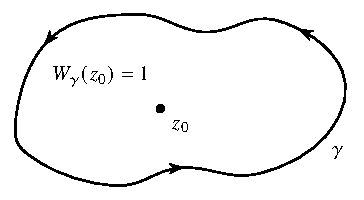
\includegraphics[width=.84\linewidth]{note5-fig-02.pdf}

  \end{minipage}
  \begin{minipage}[b]{.47\linewidth}
    \centering
    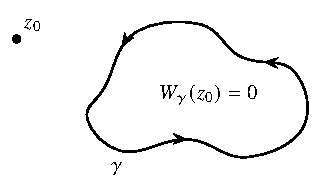
\includegraphics[width=.78\linewidth]{note5-fig-03.pdf}

  \end{minipage}
\end{figure}

We have thus far seen that \(\mathbb C\setminus\gamma([0,1])\) has at least two components, each contained in
\[
  \{z\mid W_\gamma(z)=1\}
  \quad\text{and}\quad
  \{z\mid W_\gamma(z)=0\}.
\]
Assume \(\gamma\) to be a simple closed curve. The essential question we now ask is: how many components does \(\mathbb C\setminus\gamma([0,1])\) have? We know that there are at least two. The \emph{Jordan Curve Theorem} states that there are exactly two. That is, the sets
\[
  \{z\mid W_\gamma(z)=1\}
  \quad\text{and}\quad
  \{z\mid W_\gamma(z)=0\}
\]
are connected. It is easy to see that \(\{z\mid W_\gamma(z)=0\}\) is the unbounded component, or the exterior.

Thus, \(W_\gamma(z_0)\) knows where \(z_0\) belongs. Hence, if \(\gamma\) is a simple closed curve, then the interior of \(\gamma\) is simply connected.


\textit{Proof.}
Let \(\gamma_P\) be a polygonal path in \(\gamma\), with both curves simple and closed. We first prove that
\[
  \operatorname{int}(\gamma_P)\subset\operatorname{int}(\gamma).
\]
To contrast the triviality of this fact with the analytic complexity, we present it as follows:
\[
  \gamma_P\cap\gamma=\varnothing,
  \qquad \gamma_P\text{ is connected}.
\]
Since \(\gamma_P\subset\operatorname{int}(\gamma)\), we have \(\gamma_P\cap\operatorname{ext}(\gamma)=\varnothing\). If \(\operatorname{int}(\gamma_P)\subset\operatorname{ext}(\gamma)\), then, since \(\operatorname{ext}(\gamma_P)\) is unbounded, while \(\gamma\) is compact and hence bounded, and \(\operatorname{int}(\gamma)\) is also bounded, one has
\[
  \operatorname{ext}(\gamma_P)\cap\operatorname{ext}(\gamma)\ne\varnothing.
\]
Therefore,
\[
  \operatorname{ext}(\gamma)
  =\bigl(\operatorname{int}(\gamma_P)\cap\operatorname{ext}(\gamma)\bigr)
   \cup\bigl(\gamma_P\cap\operatorname{ext}(\gamma)\bigr)
   \cup\bigl(\operatorname{ext}(\gamma_P)\cap\operatorname{ext}(\gamma)\bigr).
\]
Note that \(\gamma_P\cap\operatorname{ext}(\gamma)=\varnothing\), and we thus have a separation of \(\operatorname{ext}(\gamma)\), which is not possible.

\begin{figure}[htbp]
  \centering
  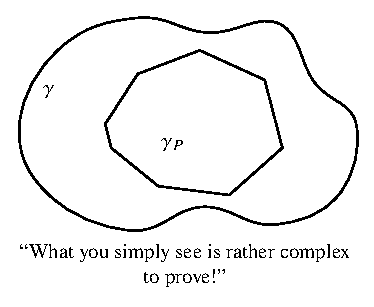
\includegraphics[width=.45\linewidth]{note5-fig-04.pdf}

\end{figure}

Now let
\[
  \operatorname{int}(\gamma_P)\cap\operatorname{ext}(\gamma)\ne\varnothing.
\]
Then \(\operatorname{int}(\gamma_P)\not\subset\operatorname{ext}(\gamma)\), so
\[
  \operatorname{int}(\gamma_P)\cap\operatorname{int}(\gamma)\ne\varnothing.
\]
Thus, \(\gamma\cap\operatorname{int}(\gamma_P)\ne\varnothing\). As \(\gamma\) is connected and \(\gamma\cap\gamma_P=\varnothing\), \(\gamma\subset\operatorname{int}(\gamma_P)\) or \(\gamma\subset\operatorname{ext}(\gamma_P)\). Since \(\gamma\cap\operatorname{int}(\gamma_P)\ne\varnothing\), \(\gamma\subset\operatorname{int}(\gamma_P).\)
Therefore,
\[
  W_{\gamma_P}(\gamma(t))=1
  \qquad(\forall t,\ t\in[0,1]),
\]
and hence \(\operatorname{ext}(\gamma_P)\cap\gamma=\varnothing\). It follows that \(\operatorname{ext}(\gamma_P)\cap\operatorname{int}(\gamma)=\varnothing\), otherwise \(\operatorname{ext}(\gamma_P)\) would have a separation. Thus,
\[
  \operatorname{ext}(\gamma_P)
  =\bigl(\operatorname{ext}(\gamma_P)\cap\operatorname{ext}(\gamma)\bigr)
  \cup\bigl(\operatorname{ext}(\gamma_P)\cap\gamma\bigr)
  \cup\bigl(\operatorname{ext}(\gamma_P)\cap\operatorname{int}(\gamma)\bigr),
\]
and therefore \(\operatorname{ext}(\gamma_P)=\operatorname{ext}(\gamma)\). Since \(W_{\gamma_P}(\gamma(t))=1\), there exists \(\varepsilon>0\) such that, for every \(z\in B_\varepsilon(\gamma(t))\), \(W_{\gamma_P}(z)=1\). Thus,
\[
  \operatorname{int}(\gamma_P)\cap\operatorname{ext}(\gamma)\ne\varnothing
  \Longrightarrow
  \operatorname{int}(\gamma_P)\cap\operatorname{ext}(\gamma_P)\ne\varnothing,
\]
a contradiction. Hence,
\[
  \operatorname{int}(\gamma_P)\cap\operatorname{ext}(\gamma)=\varnothing,
  \qquad
  \operatorname{int}(\gamma_P)\cap\gamma=\varnothing.
\]


Therefore, \(\operatorname{int}(\gamma_P)\subset\operatorname{int}(\gamma).\)
Now take any point in \(\operatorname{int}(\gamma_P)\), say \(z_0\). Notice that the straight-line path fails to be the candidate because the polygon can be concave. Thus, one must find a way to smooth off these concavities. To do that, one must ask for a classic theorem in polygon theory.

\subsection*{Two-Ears Theorem}
An ear is a vertex such that the segment between the vertices adjacent to the vertex is in the polygon. The theorem states that every simple polygon has at least two ears.

Thus, for our purposes, note that given \(\gamma_P\), there exist vertices \(v_1,v_2\) of \(\gamma_P\) such that \(\gamma_{v_1\to v_2}\subset\operatorname{int}(\gamma_P)\). Now one can induct on the number of edges. Every triangle, being convex, can be ``contracted'' to any one of its edges via a straight-line homotopy.

\begin{figure}[htbp]
  \centering
  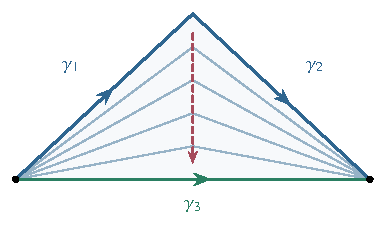
\includegraphics[width=.48\linewidth]{note5-fig-05.pdf}

\end{figure}

The homotopy
\[
  H(s,t):=(1-s)(\gamma_1+\gamma_2)(t)+s\gamma_3(t)
\]
takes \(\gamma_1+\gamma_2\) to \(\gamma_3\).

Now assume it is true for all polygons with fewer than \(N\) edges. Let \(\gamma_P\) be a polygon with \(N\) edges. We know all polygons with fewer than \(N\) edges can be deformed to any one of their edges. Using the Two-Ears Theorem, split the polygon into two, \(\gamma_{P'}\) and a triangle, with \(\gamma_{a\to b}\) the common edge. Contract \(\gamma_{P'}\) to the edge \(\gamma_{a\to b}\), and similarly do the same for the triangle. If \(H(s,t)\) and \(H'(s,t)\)


denote these homotopies, then \(H(s,t)+H'(s,t)\) is the required one.

Therefore, what we essentially proved is that polygons are null-homotopic because segments are null-homotopic, being a degenerate convex set.

Now let \(\gamma_P\) be any closed polygonal curve. Again, one can write it as a union, or concatenation, of simple closed polygonal curves. Here too, by contracting each \(\gamma_{P_i}\) in
\[
  \gamma=\sum_{i=1}^N\gamma_{P_i}
\]
to the common point, and using the fact that domains are path-connected, one can conclude the theorem for any closed polygonal path.

Now, given any general closed curve, appeal to the complex tube lemma to get a closed polygonal curve and conclude that \(\operatorname{int}(\gamma)\) is simply connected.

Here is how these deformations look:

\begin{figure}[htbp]
  \centering
  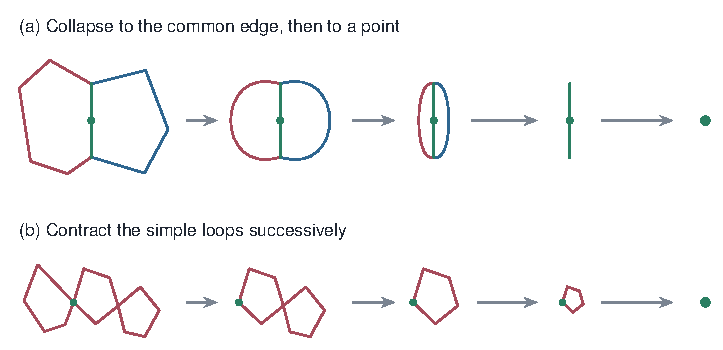
\includegraphics[width=.90\linewidth]{note5-fig-06.pdf}

\end{figure}


Therefore, \(\gamma_2\) avoids the interior of \(\gamma_1\), \(\gamma_1\) avoids the exterior of \(\gamma_2\), and the two curves are disjoint. Show that
\[
  \operatorname{int}(\gamma_2)\subset\operatorname{ext}(\gamma_1)
  \quad\text{and}\quad
  \operatorname{ext}(\gamma_2)\supseteq\operatorname{int}(\gamma_1).
\]

\textit{Proof.}
The argument in this case too is very similar to what we gave previously. We have
\[
  \gamma_1\cap\gamma_2=\varnothing,
  \qquad
  \gamma_2\cap\operatorname{int}(\gamma_1)=\varnothing,
\]
so \(\gamma_2\subset\operatorname{ext}(\gamma_1)\).

\begin{figure}[htbp]
  \centering
  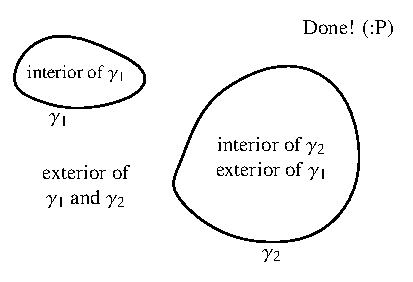
\includegraphics[width=.46\linewidth]{note5-fig-07.pdf}

\end{figure}

Since \(\operatorname{ext}(\gamma_2)\) and \(\operatorname{ext}(\gamma_1)\) are unbounded, we have
\[
  \operatorname{ext}(\gamma_2)\cap\operatorname{ext}(\gamma_1)\ne\varnothing.
\]
Also, \(\gamma_1\subset\operatorname{ext}(\gamma_2)\), so \(\gamma_1\cap\operatorname{int}(\gamma_2)=\varnothing\). If \(\operatorname{int}(\gamma_2)\subset\operatorname{int}(\gamma_1)\), then \(\operatorname{ext}(\gamma_1)\cap\operatorname{int}(\gamma_2)=\varnothing\), and hence
\[
  \operatorname{int}(\gamma_2)
  =\bigl(\operatorname{int}(\gamma_2)\cap\operatorname{int}(\gamma_1)\bigr)
  \cup\bigl(\operatorname{int}(\gamma_2)\cap\gamma_1\bigr)
  \cup\bigl(\operatorname{int}(\gamma_2)\cap\operatorname{ext}(\gamma_1)\bigr),
\]
which gives \(\operatorname{int}(\gamma_2)=\operatorname{int}(\gamma_1)\). Now
\[
  \operatorname{ext}(\gamma_2)\cap\operatorname{int}(\gamma_2)=\varnothing
  \Longrightarrow
  \operatorname{ext}(\gamma_2)\cap\operatorname{int}(\gamma_1)=\varnothing.
\]
Thus,
\[
  \operatorname{ext}(\gamma_2)=\gamma_1\cup\operatorname{ext}(\gamma_1).
\]
Inspect neighborhoods of \(\gamma_1(t)\) to get that
\[
  \operatorname{ext}(\gamma_2)\cap\operatorname{int}(\gamma_1)\ne\varnothing,
\]
which is not possible. Now, if
\[
  \operatorname{int}(\gamma_2)\cap\operatorname{int}(\gamma_1)\ne\varnothing,
\]
then, since \(\gamma_1\cap\gamma_2=\varnothing\), \(\operatorname{int}(\gamma_2)\not\subset\operatorname{int}(\gamma_1)\), so
\[
  \operatorname{int}(\gamma_2)\cap\operatorname{ext}(\gamma_1)\ne\varnothing.
\]
Therefore \(\operatorname{int}(\gamma_2)\cap\gamma_1\ne\varnothing\), but \(\gamma_1\subset\operatorname{ext}(\gamma_2)\), a contradiction. Hence,
\[
  \operatorname{int}(\gamma_2)\subset\operatorname{ext}(\gamma_1),
\]
and similarly \(\operatorname{int}(\gamma_1)\subset\operatorname{ext}(\gamma_2)\).

\subsection*{Tool 20 — Differentiation under the Integral Sign}
If \(f\) is \(C^1\), one can differentiate \(f\) under the integral sign. Therefore, \(W_\gamma(z_0)\) is locally constant.


\textit{Proof.}
Let us differentiate \(W_\gamma(z_0)\).


\[
  \frac{d}{dz_0}\left(\frac{1}{2\pi i}\int_\gamma\frac{dz}{z-z_0}\right)
  =\frac{1}{2\pi i}\int_\gamma\frac{d}{dz_0}\left(\frac{1}{z-z_0}\right)\,dz,
\]
where \(\gamma\) is a circle here. Hence,
\[
  \frac{1}{2\pi i}\int_\gamma\frac{dz}{(z-z_0)^2}=0
\]
by the higher-order Cauchy Integral Formula. Therefore,
\[
  \frac{d}{dz_0}W_\gamma(z_0)=0,
\]
so \(W_\gamma(z_0)\) is locally constant.

\textbf{Note.}
We have seen many instances of Tool 20 before. Finally, it made the list too!

\subsection*{Fundamental Theorem of Algebra (again)}
Let
\[
  P(z)=\sum_{n=0}^N a_nz^n
\]
be a polynomial with \(a_i\in\mathbb C\). Let \(\gamma_R:[0,2\pi]\to\mathbb C\) be the closed contour
\[
  \gamma_R(t):=P(Re^{it}).
\]
Note that, for \(R\) large enough,
\[
  |R^ne^{int}a_n|>
  \left|\sum_{n=0}^{N-1}R^ne^{int}a_n\right|.
\]
It dominates by the triangle inequality:
\[
  |R^ne^{int}a_n|>
  \sum_{n=0}^{N-1}|R^ne^{int}a_n|,
\]
which dominates
\[
  \left|\sum_{n=0}^{N-1}R^ne^{int}a_n\right|.
\]
This also means that the contours \(R^ne^{int}a_n\) and \(P(Re^{it})\) share the same winding number around \(0\), because
\[
  |R^ne^{int}a_n-0|>|R^ne^{int}a_n-P(Re^{it})|
  \qquad(\forall t).
\]
Therefore,
\[
  W_{R^ne^{int}a_n}(0)=W_{P(Re^{it})}(0)
  =\frac{1}{2\pi i}\int_0^{2\pi}
    \frac{R^nina_ne^{int}}{R^ne^{int}a_n}\,dt
  =n.
\]
Recall that, via this technique of local constancy, we established the notion of interior and exterior. Now, if \(P\) does not vanish on \(\overline{B_R(0)}\), then we have
\[
  \frac{1}{2\pi i}\int_{P\circ Re^{it}}\frac{dz}{z}
  =\frac{1}{2\pi i}\int_{Re^{it}}\frac{P'(z)}{P(z)}\,dz=0.
\]
This contradicts local


constancy. Therefore, \(P(z)\) has zeros on a large enough disc.

\subsection*{Higher-Order Cauchy Integral Formula}
\[
  W_\gamma(z_0)f^{(n)}(z_0)
  =\frac{n!}{2\pi i}\int_\gamma\frac{H(z)}{(z-z_0)^{n+1}}\,dz.
\]
The derivative of \(W_\gamma(z_0)\) is \(0\), since \(W_\gamma(z_0)\) is locally constant. Thus,
\[
  \frac{d}{dz_0}\bigl(W_\gamma(z_0)f(z_0)\bigr)
  =\frac{d}{dz_0}\left(\frac{1}{2\pi i}\int_\gamma\frac{dz}{z-z_0}\right)H(z_0)
   +W_\gamma(z_0)f'(z_0).
\]
Also,
\[
  \frac{d}{dz_0}\left(\frac{1}{2\pi i}\int_\gamma\frac{H(z)}{z-z_0}\,dz\right)
  =\frac{1}{2\pi i}\int_\gamma
    \frac{d}{dz_0}\left(\frac{H(z)}{z-z_0}\right)\,dz.
\]
Therefore,
\[
  W_\gamma(z_0)f'(z_0)
  =\frac{1}{2\pi i}\int_\gamma\frac{H(z)}{(z-z_0)^2}\,dz.
\]
One can now finish the argument via induction.

\textbf{Remark.}
Note that all finite field extensions of \(\mathbb R\) are quotients of \(\mathbb R[x]\). They are of the form \(\mathbb R[x]/(P(x)),\)
where \(P\) is irreducible in \(\mathbb R\). We saw that \(P(x)\) has a root in \(\mathbb C\). Observe that if
\[
  P(z_0)=\sum_{n\ge0}a_nz_0^n=0,
\]
then
\[
  \overline{P(z_0)}=\sum_{n\ge0}\overline{a_n}\,\overline{z_0}^{,n}
  =P(\overline{z_0})=0.
\]
Hence, \(\overline{z_0}\) is a root if \(z_0\) is a root, and
\[
  (z-z_0)(z-\overline{z_0})\mid P(z).
\]
If \(\deg(P)>2\), then \(P\) is reducible, which is not possible. Thus \(\deg(P)=2\), so
\[
  P(z)=az^2+bz+c.
\]
Completing the square, under a suitable linear transform, \(P(z)=z^2+a^2.\)
Therefore,
\[
  \mathbb C\cong\mathbb R(\sqrt{-a})
  \cong\mathbb R(\sqrt a,\sqrt{-1})
  \cong\mathbb R(\sqrt{-1})
  \cong\mathbb C.
\]
Thus, \(x^2+1\) is the natural


choice that there is. The field we constructed is one of its kind!

To be in a position to procure as much geometric information stored in the regularity of a holomorphic function, one must be sound with deformations of curves, because, as we recently saw, one can integrate our holomorphic function on any continuous curve. Moreover, if two curves are homotopic, with the homotopy in the domain of holomorphy of \(f\), then the value of the integral slides via the homotopy from one curve to the other without any change.
% BLOG-CONTENT-END
\end{document}
